\documentclass[dvipdfmx]{article}
\usepackage[dvipdfmx]{graphicx}
\usepackage{amsmath, amssymb}
\usepackage{mathtools}
\usepackage{here}
\usepackage{svg}

\begin{document}
\title{Weekly Report}
\author{Riku Gondow}
\maketitle
\section{Progress}
\begin{itemize}
    \item Check accuracy using EMD in close set 
    \begin{itemize}
        \item The accuracy was 29.83\%. So the result wasn't better than just using BPF without EMD.
    \end{itemize} 
\end{itemize}

\begin{figure}[H]
\begin{center}
\includegraphics[width=0.7\linewidth]{./img/conf_emd.png}
\end{center}
\caption{Confusion Matrix of the method with EMD}
\end{figure}

\section{Problem when using EMD}
If there is a large peak in the segment, it appears that the EMD is not working effectively as shown in Figure2. Therefore, peak detection should be performed to remove those peaks. Peak removal may contribute to learning stability even when not using EMD.

\begin{figure}[H]
    \begin{center}
    \includegraphics[width=0.5\linewidth]{./img/peak_wave.png}
    \end{center}
    \caption{An example of an EMD segment including a large peak}
    \end{figure}

\begin{figure}[H]
\begin{center}
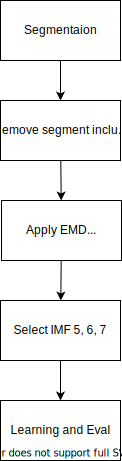
\includegraphics[width=0.5\linewidth]{"./img/flowchart.png"}
\end{center}
\caption{Preprocessing algorithm with Peak Detection}
\end{figure}

\section{Next Plan}
\begin{itemize}
    \item Check accuracy with EMD and Peak detection
    \item Use EEMD for preprocessing
    \item Prepare presentation
\end{itemize}

\end{document}